\documentclass[a4paper, 12pt]{article}

\usepackage{graphicx}
\usepackage[font=small, labelfont=bf, labelsep=colon]{caption}
\usepackage{amsmath, amssymb}
\usepackage{float}
\usepackage{comment}
%\usepackage{textcomp}
%\usepackage{siunitx}
\usepackage[dvipsnames]{xcolor}
%\usepackage{ctable}
%\usepackage{multirow}
\usepackage[flushmargin, bottom]{footmisc} 
\usepackage{hyperref}

%\hypersetup{
%colorlinks = true,
%linkcolor = {blue!80!black}
%}

\graphicspath{{../Pictures/}}

%%%%%%%%%%%%%%%%%%%%%%%%%%%%%%%%%%%%%%%%%%%%%%%%%%%%%%%
% Layout parameters 
\setlength{\parindent}{0em}
\setlength{\parskip}{2ex}
\linespread{1.2}

\renewcommand{\floatpagefraction}{.99} % Minimum fraction of floats, in a page that has only floats. Only figures taking up more than that will get their own page. Default 0.5
\renewcommand{\topfraction}{0.99}  % Maximum fraction of page for floats at top. I.e.: floats taking up more than this will have no text below. Default: 0.7.
\renewcommand{\textfraction}{0.01} % Minimum fraction of page that must have text (otherwise, the page will only have float). Default: 0.2 

\addtolength{\textwidth}{2cm}
\addtolength{\hoffset}{-1cm}
\setlength{\topmargin}{-1cm}
\addtolength{\textheight}{1cm}

\setlength{\skip\footins}{6mm} % space between end of text and horizontal line of footnote
\setlength{\footnotesep}{5mm} % space between footnote line and first entry, and between consecutive entries of footnote



%%%%%%%%%%%%%%%%%%%%%%%%%%%%%%%%%%%%%%%%%%%%%%%%%%

%%%%%%%%%%%%%%%%%%%%%%%%
%%%%% NEW COMMANDS
%%%%%%%%%%%%%%%%%%%%%%%%

% Text commands
\newcommand{\spc}{1ex}
\newcommand{\eg}{\textit{e.g.}}
\newcommand{\ie}{\textit{i.e.}}
\newcommand{\red}{\textcolor{red}}

% Maths Commands



%%%%%%%%%%%%%%%%%%%%%%%%%%%%%%%%%%%%%%%%%%%%%%%%%%%%%

\title{(Very!) Preliminary Report - ColaLife Project}

\author{}
\date{}

\begin{document}

\maketitle


\section{Methods}

\subsection{The context}

\subsection{Data Collection}
Our objective was to compare dispensing practices in government health facilities on the frontline of primary healthcare in Mongu District before co-packaged ORS and zinc was introduced, in 2016, and after it was available, in 2017. We selected the month of October to make this comparison as it is the peak month for diarrhoea cases. We determined that in order to make this comparison all dispensing options needed to be available and in stock: ORS and zinc (packed separately) in 2016, and ORS and zinc (packed separately) as well as co-packaged ORS and zinc in 2017. We did not influence the normal stocking procedures of the Ministry of Health to undertake this study. Instead, we surveyed 29 frontline health facilities in the district to assess the stock status of separately packaged ORS and zinc in October 2016, and of ORS, zinc and the new co-packaged ORS and zinc product in October 2017. In this process we identified five facilities with inadequate stock records and these were excluded from future consideration. A fully stocked facility was defined as one which had records of stock of all dispensing options at both the beginning and end of October in both 2016 and 2017. Nine of the 24 facilities met these stocking criteria. However, we had the operational resources to visit seven of these (see Figure 3), and these form the source of the data used within this study. All dispensing data were collected by a single enumerator between 23 Nov 2017 and 28 Dec 2017.

The enumerator used the existing Health Ministry dispensing ledger to establish actual dispensing behaviour, recording it on a paper-based tally sheet. A bespoke tablet-based form developed in CommCare was used to collect general data about each facility and the tablet’s GPS capability collected the facility’s location. At the end of the process a picture was taken of the two tally sheets, one for 2016 and one for 2017, and these were uploaded to the server through the CommCare form. 


\subsection{Statistical Methods}

The main indicator of interest throughout this study is the probability with which both ORS and zinc are dispensed at a health facility, whether co-packaged or not, as diarrhoea treatment for a child under the age of 5 years. We denote by $p_1$ its value before the co-pack introduction, and by $p_2$ its value after the co-pack introduction. Although both probabilities are unknown, the available data can be employed to estimate each of the two and their difference/ratio with a given confidence, and more generally to carry out statistical analyses to address the question that $p_2 > p_1$.
In the following we use the acronym CDCs (correctly-dispensed cases) to refer succinctly to those cases where both ORS and zinc were dispensed as diarrhoea treatment, either packaged individually (the only option in 2016) or as a co-pack.

\subsubsection{Analysis on Individual and Agglomerated Data}

In any given context (whether concerning a single health facility or the aggregated data), the relationship between the availability of the co-pack and the dispensing behaviour can be summarised by a 2x2 contingency table:
 
 \begin{center}
 \begin{tabular}{c|cc}
 & \bf Before Co-pack & \bf After Co-pack \\ \hline
 \bf Correct Dispensing & a & b \\
 \bf Incorrect Dispensing  & c & d  
\end{tabular}
\end{center}

The value of each cell represents the number of cases recorded for the particular combination that the cell refers to. Through this data, we estimate the probabilities $p_1$ and $p_2$ as the proportion of CDCs within the relevant sample: 
$\hat p_1 = a/(a+c)$ and $\hat p_2 = b/(b+d)$. 
We also report the 95\% confidence interval (CI) to quantify the reliability of the estimate.
This is computed via the Clopper-Pearson method using the exact binomial distribution\cite{clopper1934}.

To test whether a significant increase in the proportion of CDCs has taken place upon introduction of the ORS and zinc co-pack, we perform a one-sided test of homogeneity of binomial proportions on the contingency table. This tests the null hypothesis that the proportions of CDCs before and after the co-pack introduction are equal to each other ($p_1=p_2$), against the alternative that the latter is higher than the former ($p_2>p_1$).

We perform all hypothesis tests in this work at the 5\% significance level: that is, the null hypothesis is rejected whenever the $p$-value is less than 0.05. The $p$-value is a measure of the probability of observing the available data, if the null hypothesis was true. Thus,
small $p$-values, especially notably smaller than 0.05, represent strong evidence against the null hypothesis, and in favour of the alternative.
%particularly small $p$-values indicate that the data carries strong evidence against the null hypothesis, and in favour of the alternative.
For the afore-mentioned homogeneity of proportions test, a significant $p$-value indicates an increase in the proportion of CDCs after the co-pack introduction, but it does not quantify the effect of the latter on the proportion of CDCs. To this purpose, we employ i) the difference between the two proportions and ii) the rate ratio. 

The difference between the two proportions is estimated via the sample difference and its $95\%$ Wald CI \cite{agresti2002}, constructed using the large-sample normal approximation for the difference of binomial distributions. 
% and provides a range of values that are expected to contain the true difference between the two proportions, with 95\% confidence. 
The rate ratio is instead computed as the ratio between the proportions of CDCs after co-pack introduction, and the proportion before co-pack introduction ($p_2/p_1)$. It quantifies how many times more (or less) likely a child is to receive the correctly-dispensed treatment for diarrhoea after the co-pack introduction, than before. A CI for the rate ratio is provided, following the method cited \cite{agresti2002, nam1995}.

\subsubsection{Controlling for Data Stratification}

The previous measures and statistical tests can be performed at the level of a single health facility or of the pooled data. The last option provides an overall picture and generally improves statistical significance due to a larger sample size. However, it disregards the stratification of the original data across the facilities. To test for a relationship between the introduction of co-packaging and the proportion of CDCs, while controlling for the stratification of the data, we employ the Mantel-Haenszel test.
The test uses the odds ratio as a measure of the association between dispensing behaviour and the introduction of the co-pack. We briefly recall below the meaning of odds and odds ratios, with specific reference to our context.

%The previous measures and statistical tests analyse the relationship between two binary variables (presence/absence of co-pack and correct/incorrect dispensation). They can be  performed at the level of a single health facility or of the pooled data. The last option has the advantage of providing an overall picture and generally improving statistical significance due to a larger sample size. However,  the methods disregard the stratification of the original data across the facilities. To test for a relationship between the introduction of co-packaging and the proportion of CDCs, while controlling for the stratification of the data across different facilities, we employ the Mantel-Haenszel test.

In each of the two co-pack settings (before and after the co-pack introduction), the odds of correct dispensation are defined as the ratio between the probability of correct dispensation and the probability of incorrect dispensation: 
$$
\text{Odds}_1 = \frac{p_1}{1-p_1} 
\quad \text{ and } \quad
\text{Odds}_2 = \frac{p_2}{1-p_2}\,.
$$
Thus, they can be interpreted as the expected number of CDCs for each incorrectly-dispensed case, before and after the co-pack introduction respectively.
The odds ratio is then defined as the ratio between the odds of correct dispensation after co-pack (Odds$_2$), and the odds of correct dispensation before co-pack (Odds$_1$):
$$
\text{OR} = \frac{p_2 \times (1-p_1)}{p_1 \times (1-p_2)}\,.
$$
In the case of a single contingency table, it is easy to check that the odds ratio can be written as $\text{OR} = (bc)/(ad)$. 
In the case of a series of contingency tables (as our case is, with one table for each health facility), a common odds ratio is defined through the following formula:
\begin{equation}\label{eqn_R}
R %= \frac{\,\sum_i \frac{b_i c_i}{n_i}\,}{\sum_i \frac{a_i d_i}{n_i}}
= \frac{\,\sum (b_i c_i)/n_i\,}{\sum (a_i d_i)/n_i},
\end{equation}
where $a_i, \dots, d_i$ are the numbers in the contingency table of the $i^{th}$ health facility, and $n_i$ is their sum (the total number of cases for that facility).

Given a series of contingency tables, the Mantel-Haenszel test assumes the null hypothesis that the common odds ratio equals 1, and tests it against the available data. Under the null hypothesis, the $R$ statistics in equation~\eqref{eqn_R} follows asymptotically a $\chi^2$ distribution with 1 degree of freedom. The approximation improves as long as the total sample size increases, independently of the total number of strata \cite{agresti2002}.

In addition to performing the test, the approximating $\chi^2$ distribution also allows to generate a CI for the estimated common odds ratio. To visualise this and the odds ratios of each facility, we use a forest plot [cit].


%\subsection{Logistic Model}
%The seven centers represent in fact a random sample of centers chosen from among many more possible centers (hundreds?). 
%The seven centers represent a few (randomly selected) instances chosen from among many more possible centres.

%There will be variability among the different centers in their correct-dispensing rates, which we account for by including the sites as random effect in our model. 


\section{Results}

\subsection{Analyses of the Agglomerated Data}

Although only nine facilities met our inclusion criteria of having recorded stock of all available CDC options in both 2016 and 2017, it should be noted that in both years around twice this number of facilities were in a position to dispense both ORS and zinc (17 in 2016 and 18 in 2017), according to their stock records. See Figure 4.

For the facilities that met our inclusion criteria, the number of diarrhoea cases observed and the number of correctly-dispensed cases (CDCs) before and after the introduction of the co-pack are given in Table 1. The probability of correct dispensation before the co-pack introduction is estimated as 0.46, CI: (0.38, 0.53). After the co-pack introduction, the estimate rises 0.87, CI: (0.83, 0.90). 


Moreover, a one-sided test of homogeneity of proportions returns a highly significant $p$-value ($p<0.0001$), suggesting that the data carries strong evidence towards the hypothesis that the proportion of CDC has increased after the introduction of the co-pack.
The difference between the two proportions is estimated to be $0.41$, with a 95\% CI of $(0.33, 0.49)$.

Figure~\ref{Fig_Overall_Proportions} provides a graphical illustration of the overall position (last row) presented in Table 1.
The left panel shows the two proportions (bars) and their CIs (whiskers) on a percentage scale, while the right panel highlights the position of the 95\% CI of their difference, on a scale $-100$\% to 100\%.
It can be seen that the CIs for the two individual proportions are neatly separated from each other, suggesting that the possibility that the true proportions are equal ($p_1=p_2$) is extremely remote. This is additionally confirmed by the 95\% CI of their difference (``after co-pack'' minus ``before co-pack''), which lies entirely within the positive side of the range.


\begin{figure}
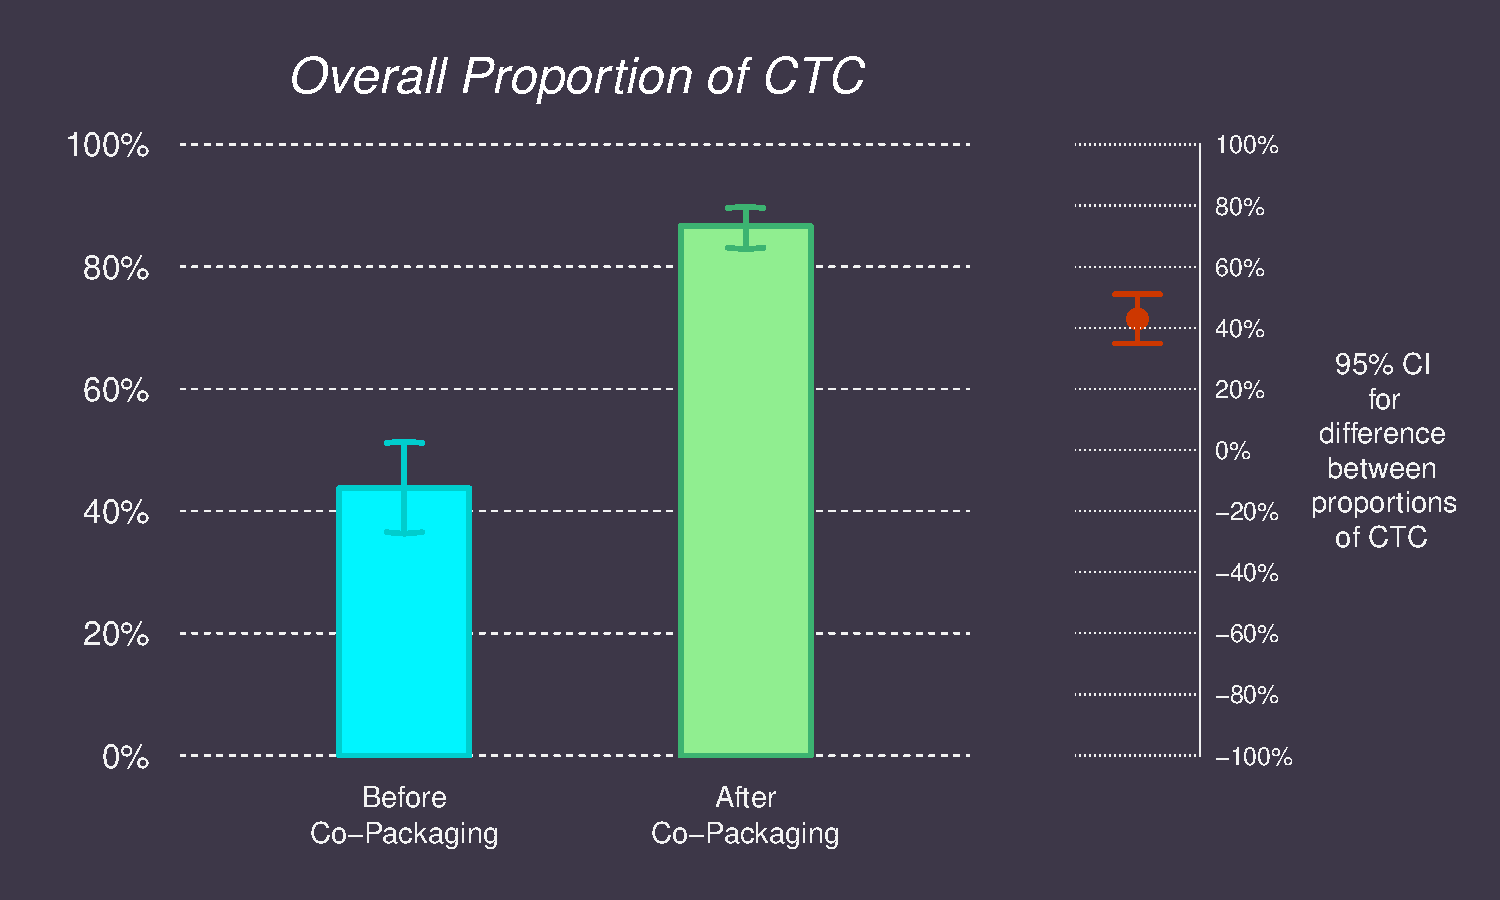
\includegraphics[width=\textwidth]{Overall_Difference_Proportions}
\caption{Comparison of the proportion of CDCs across all seven facilities, before and after co-packaged ORS and zinc was available. 
Left panel: Each of the two proportions is shown as the height of the corresponding bar, with 95\% CI (whiskers). Right panel: CI of the difference between the two proportions.}
\label{Fig_Overall_Proportions}
\end{figure}

Finally, the 95\% CI for the rate ratio of the two proportions equals $(1.62, 2.25)$. 
In other words, with 95\% confidence, we can state that
the rate of correct dispensation is between $62\%$ and $125\%$ higher after the introduction of the co-pack, than it was before.
The 99\% CI $(1.55, 2.39)$ is only slightly wider and once again reflects an increase of the
probability of correct dispensation throughout its entire range.


%%%%%%%%%%%%%%%%%%%%%%%%%%%%%%%%%%%%%%%%

%%%%%%%%%%%%%%%%%%%%%%%%%%%%%%%%%%%%%%%%


\subsection{Analyses of the Individual Facilities}
Similarly to the analysis performed on the agglomerated data, we can compute the proportions of CDCs and their CIs for each of the seven facilities, before and after the co-pack introduction. 
Figure~\ref{Fig_Single_Proportions} provides an illustration of the comparison.
As in Figure~\ref{Fig_Overall_Proportions}, the height of each bar represents the sample proportion of CDCs in the relevant case. Associated with the sample proportion is the 95\% CI quantifying the reliability of the estimate.

We note that the increase in the proportion of CDCs can be observed within each facility, 
not just in the agglomerated data as shown in Figure~\ref{Fig_Overall_Proportions}.
The amplitude of the CIs varies considerably between facilities, reflecting different sample sizes: larger sample sizes yield narrower CIs. For most facilities (five out of seven) the CIs before and after co-pack do not overlap with each other. This is a strong indication that a significant increase in the proportion of CDCs has taken place in those facilities after the co-pack introduction. 

Mulawbwa and Nalwei are the two facilities where some overlap between the two CIs can be observed. Looking at Figure~\ref{Fig_Single_Proportions}, we note that this is mainly due to the high correct-dispensing rates which the two facilities exhibit\red{ed} even prior to the co-pack introduction, differently from all other facilities. This is interesting and a point that we expand upon in the discussion.

%Mulawbwa is the only urban HC and, contextually, a significantly larger centre than the other six considered in this study. Nalwei, instead, is a RHC, however it is the closest to Mongu town. Hence, the data provides a suggestion that the greatest effect of co-packaging on dispensing behaviour is observed in those centers farthest from town. We speculate that a possible reason for this is that the latter may not be well-stocked and are often staffed by personnel with little to no medical training. Thus, the advantage of having a single co-pack ready to be dispensed when presented with a diarrhoea case may be most evident in these contexts (also ``realities'' may be a good term? Not sure, you native speakers decide :)).

Despite the partial overlap of the two CIs for Mulambwa, we note that the increase in the proportion of CDCs is significant for this facility, as revealed by the entirely positive 95\% CI for the difference of proportions: $(0.014, 0.257)$. The 95\% CI for Nalwei does instead include 0, $(-0.08, 0.41)$: i.e., for this facility, we do not have enough evidence to infer a significant increase in the proportion of CDCs, following the co-pack introduction. 

\begin{figure}
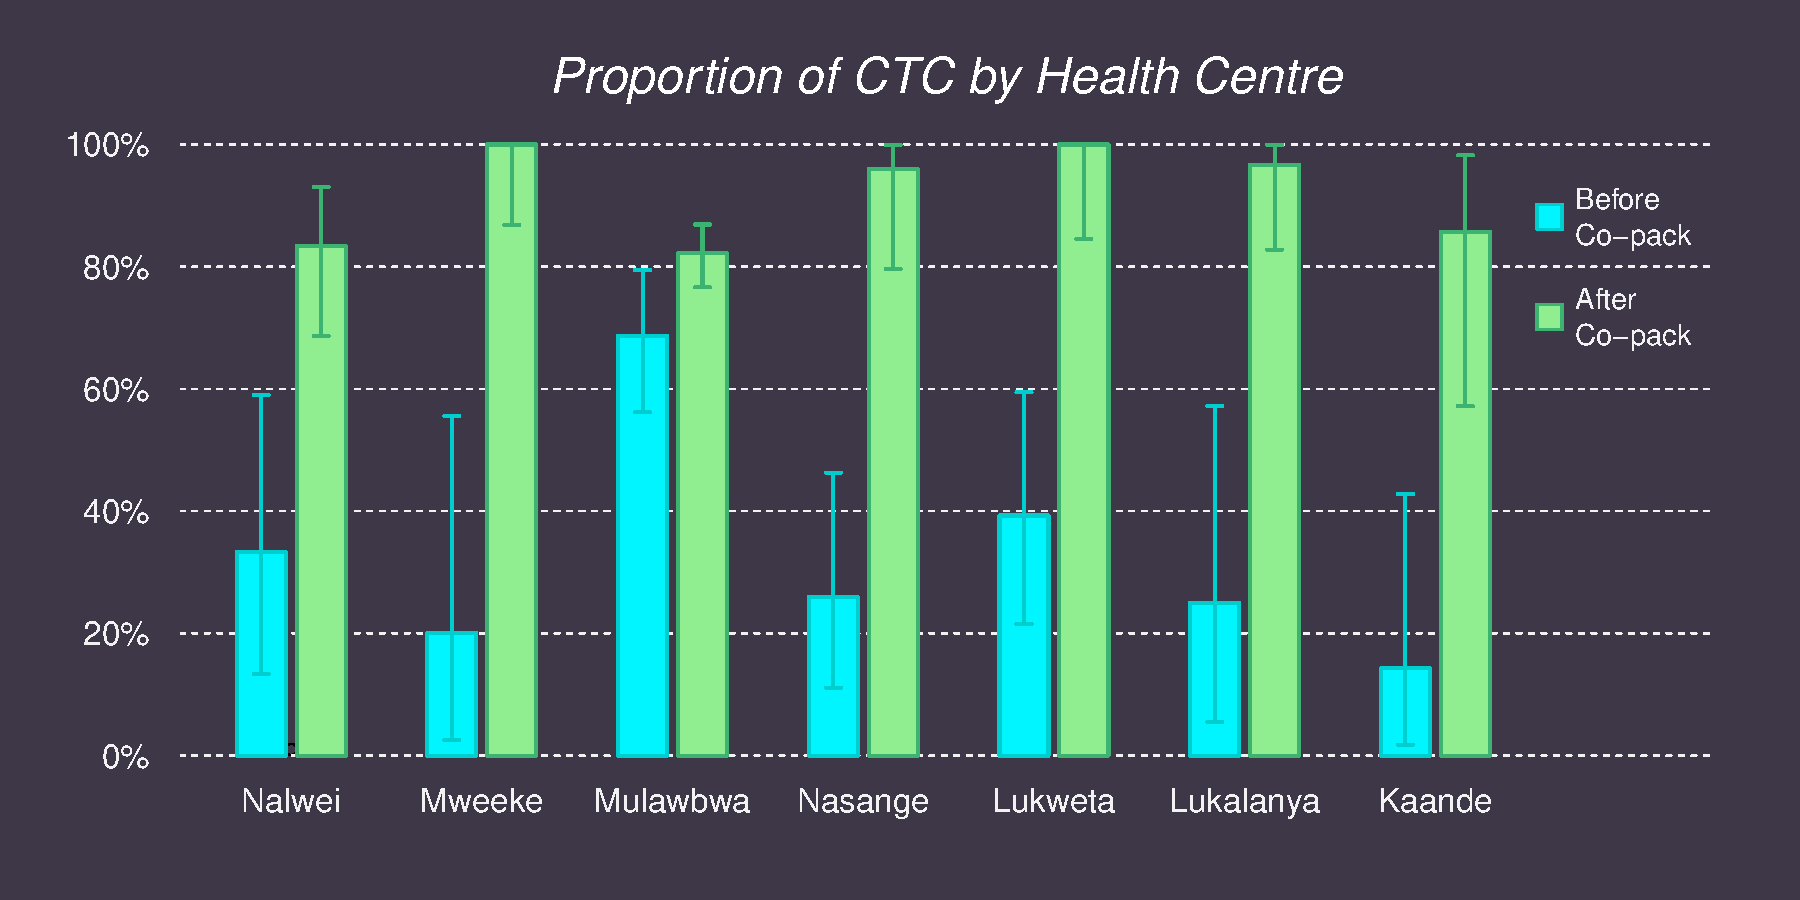
\includegraphics[width=\textwidth]{HC_Proportions}
\caption{Comparison of the proportion of CDCs before and after co-packaging, for each of the seven health facilities. The sample proportion in each case is represented by the height of each bar, while the whiskers identify the associated 95\% CI.}
\label{Fig_Single_Proportions}
\end{figure}

To test for an increase in the common odds ratio (OR), while controlling for the stratification of the overall data across the seven facilities, we perform the Mantel-Haenszel test. The test returns a highly significant result ($\chi_1^2=91.51$, $p<0.001$), with an estimated common OR equal to $6.47$ and associated 95\% CI $(4.33, 9.68)$. The result therefore suggests that the odds of correct dispensation have at least quadruplicated after the introduction of the co-pack.

The common OR and its CI are shown in the forest plot in Figure~\ref{Fig_FP}, together with the OR of each individual facility. It can be noticed that all sample ORs are higher than 1, and almost all have a 95\% CI lying entirely to the right of 1. Once again, the same five facilities show the greatest increase in their odds of correct dispensation after the introduction of the co-pack (\textit{i.e.}, the largest ORs), while the improvement in Mulambwa UHC and Nalwei HP is present but more contained. Overall though, the improvement is highly significant, as revealed by the position of the green diamond in the last row.



\begin{figure}
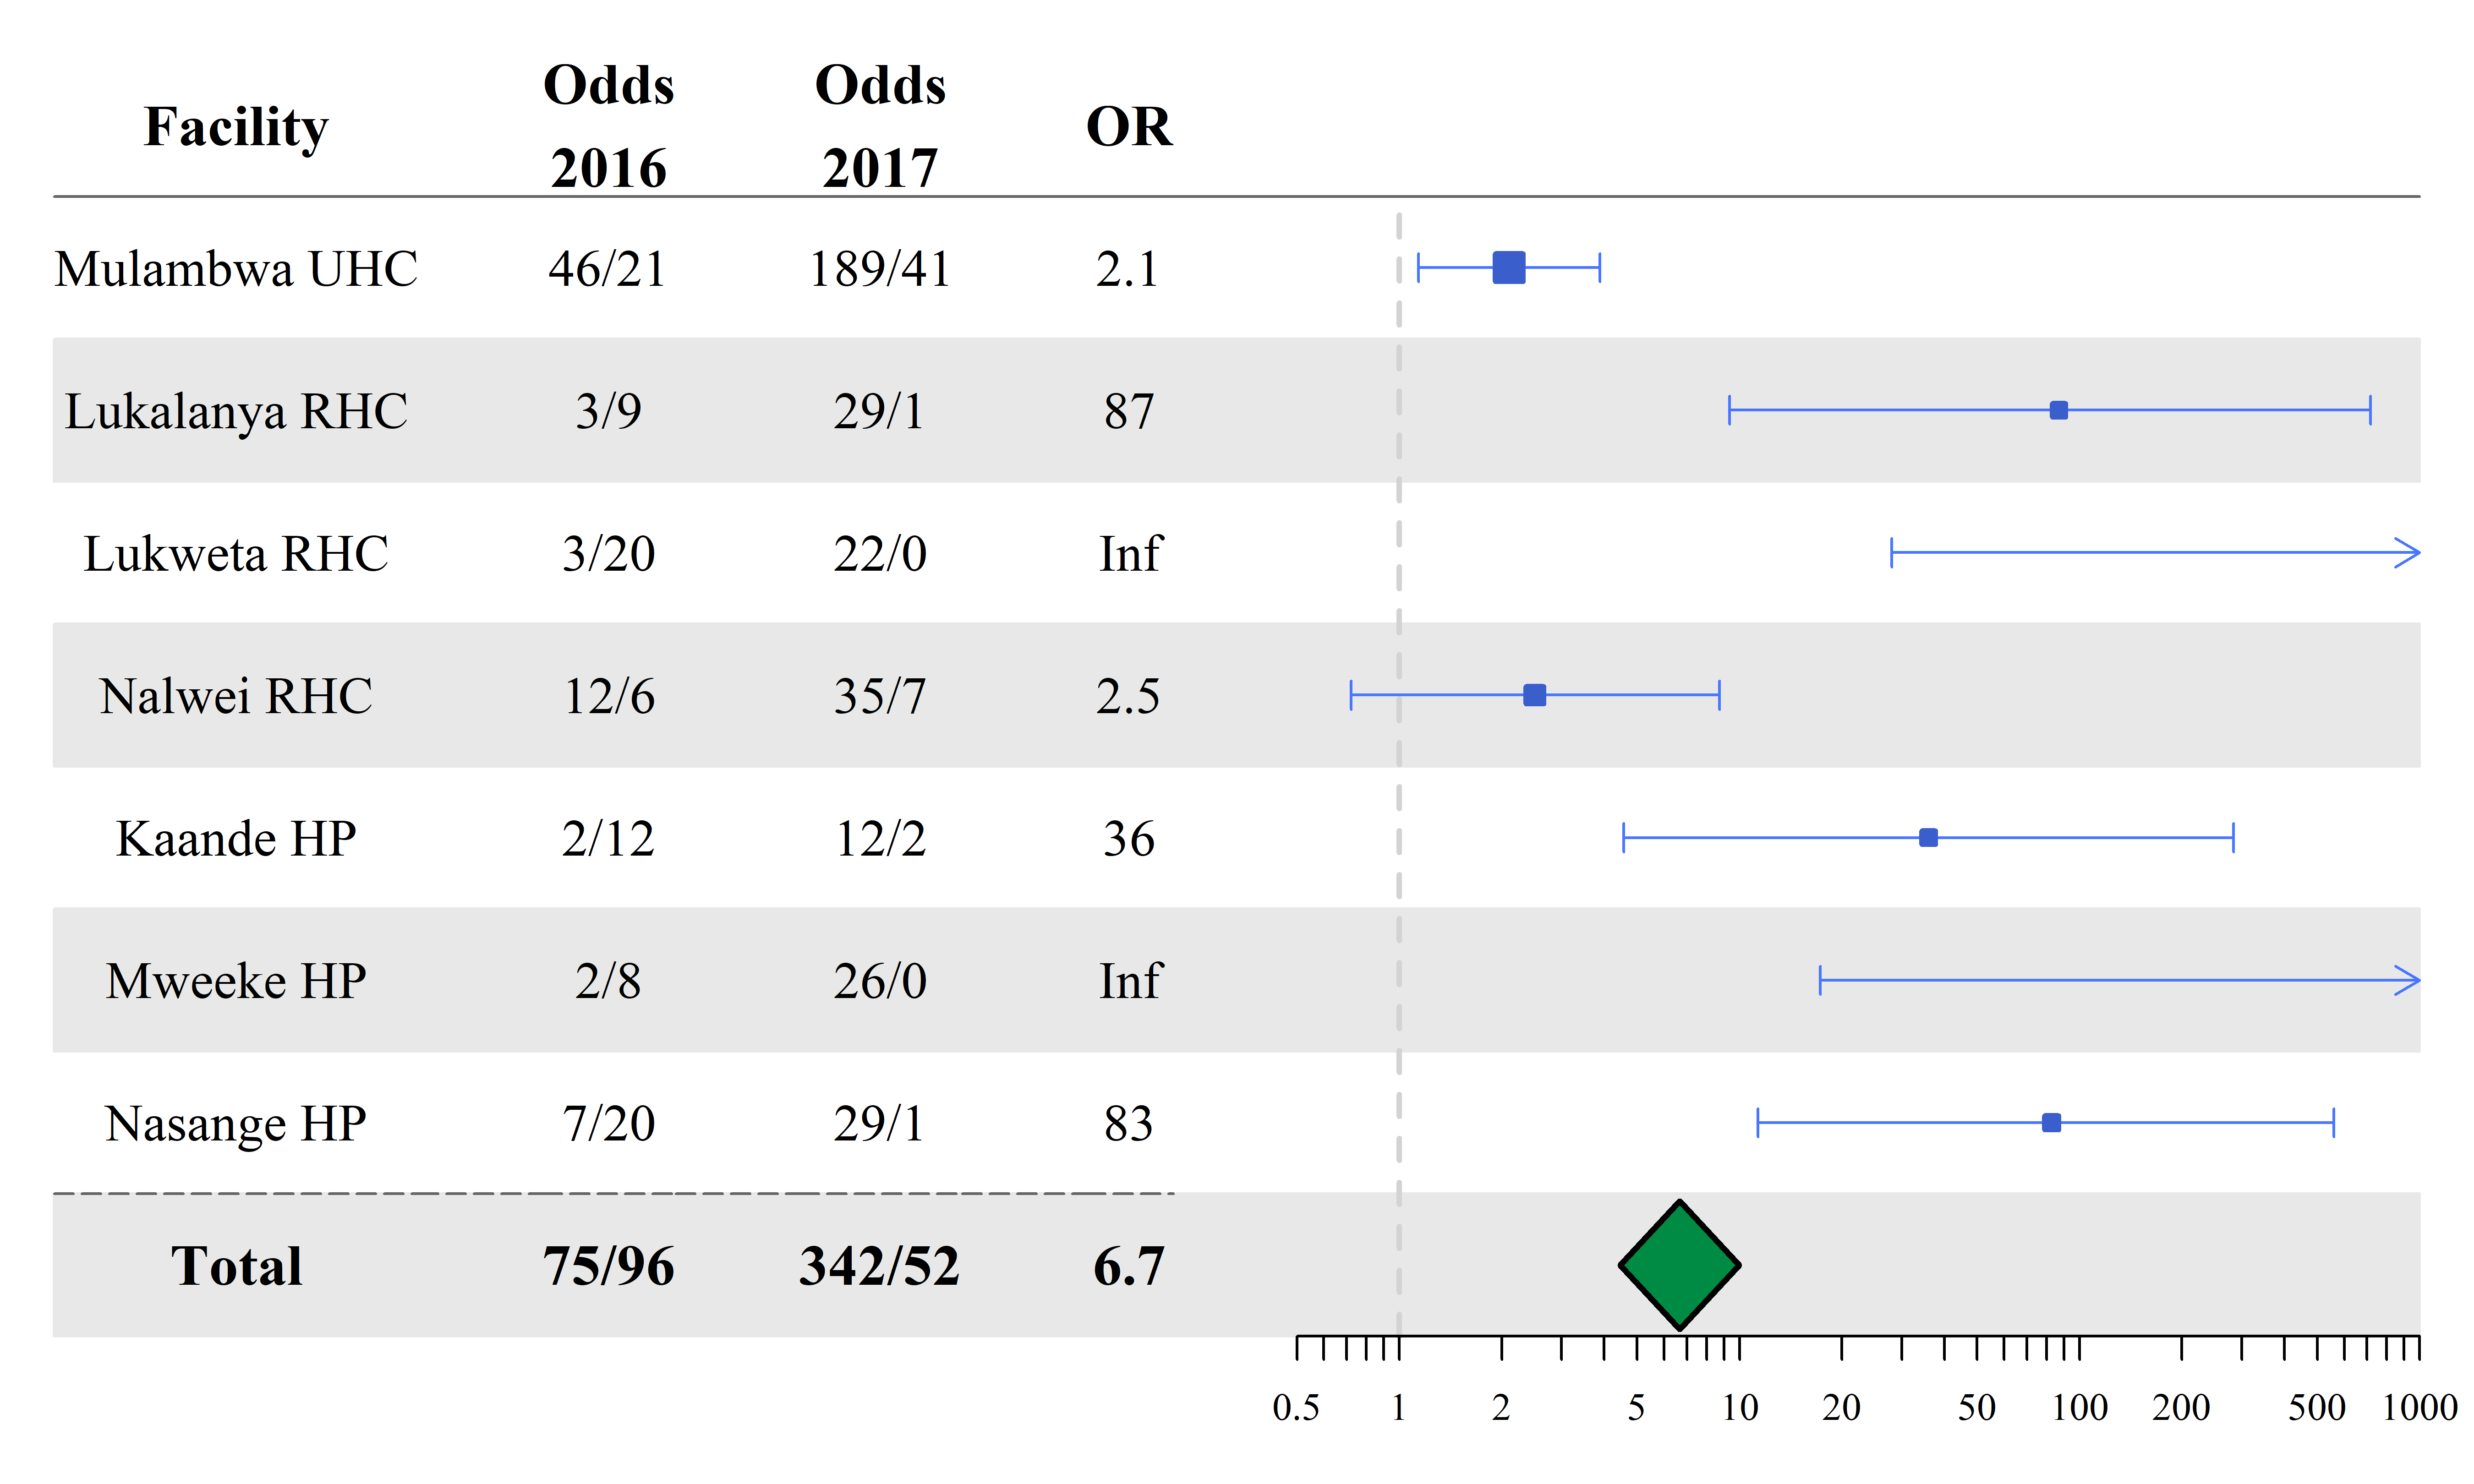
\includegraphics[width=\textwidth]{ForestPlot.png}
\caption{Odds and odds ratio (OR) for the seven health facilities. Blue squares identify the OR, whiskers the 95\% CI, the vertical line at 1 the line of no association between co-packaging and correct dispensing behaviour. The area of each square is proportional to the sample size of the facility. Last row: OR and its 95\% CI (left and right side of the green diamond) for the overall data, estimated through the Mantel-Haenszel test (equation~\eqref{eqn_R}). 
Note: for Mweeke HP, the absence of incorrectly-dispensed cases in 2017 yields an infinite OR in the sample.}
\label{Fig_FP}
\end{figure}




\newpage
\bibliographystyle{unsrt} 
\bibliography{References}  




\end{document}
